%%%%%%%%%%%%%%%%%%%%%%%%%%%%%%%%%%%%%%%%%%%%%%%%%%%%%%%%%%%%%%%%%%%%%%%%%%%%%%%%
% ICRA 2027 -- Mapless Stabilizing Anti-Stuck Flipper Control (double-blind submission)
% ICRA 2026/2027 format: standard IEEE conference template (IEEEtran),
% US-letter, two-column, 8 pages incl. references.
%%%%%%%%%%%%%%%%%%%%%%%%%%%%%%%%%%%%%%%%%%%%%%%%%%%%%%%%%%%%%%%%%%%%%%%%%%%%%%%%
\documentclass[conference]{IEEEtran}
\IEEEoverridecommandlockouts

\usepackage{cite}               % IEEE-standard compressed multi-cites: sorted, consecutive collapse to ranges like [1]-[3]
\usepackage{amsmath,amssymb,amsfonts}
\usepackage{algorithmic}
\usepackage{graphicx}
\usepackage{pgfplots}\pgfplotsset{compat=1.18}
\usepackage{booktabs}
\usepackage{array}
\usepackage{multirow}
\usepackage{subcaption}
\usepackage{xcolor}
\usepackage{siunitx}
\usepackage[hidelinks]{hyperref}
\usepackage{needspace}          % keep "Contributions:" heading with its list across a column break

% Simple inline draft marker (no todonotes dependency; safe in two-column).
\newcommand{\TODO}[1]{\textcolor{red}{\textbf{[TODO: #1]}}}
\newcommand{\placeholder}[1]{\textcolor{gray}{#1}}

\newcommand{\GC}{GC}
\newcommand{\OA}{OA}
\newcommand{\SAS}{SAS}                    % Stabilizing Anti-Stuck (our method, mode 12)
\newcommand{\cmark}{\checkmark}
\newcommand{\xmark}{\ensuremath{\times}}

\begin{document}

\title{Mapless Stabilizing and Anti-Stuck Flipper Control\\ for Articulated Tracked Robots}
% Alternative titles
% Get Unstuck Without a Map: Proprioceptive Stabilized Anti-Stuck Flipper Control
% When the Map Fails: Mapless Flipper Control for Articulated Tracked Robots
% Proprioceptive Flipper Control: Attitude-Stabilized Anti-Stuck Without a Terrain Map

% Double-blind review: author block and funding acknowledgement removed.
% Restore for the camera-ready version from git history (commit before the anonymization).
\author{\IEEEauthorblockN{Anonymous Authors}}

\maketitle

\begin{abstract}
Nearly every autonomous or semi-autonomous flipper controller assumes access
to an \emph{elevation map} of the ground under and in front of the robot. Because the terrain
beneath the chassis is occluded from the robot's exteroceptive sensors, this map cannot
be measured directly; it must be estimated from earlier observations and odometry integration, whose drift corrupts it. We present
\emph{Stabilizing Anti-Stuck} (\SAS),
a mapless, localization-free controller that combines a stabilization term for body roll
and pitch with an anti-stuck term that frees the robot when it is stuck. \SAS{} uses as input the IMU, the flipper joint angles, the commanded
velocity, and a short-window odometry cue. We deploy \SAS{} on a tracked robot with four flippers and evaluate it against manual
teleoperation and prior flipper controllers in a large comparison run, both in Gazebo
and in a real automated obstacle arena. In simulation and on the real robot, \SAS{} reaches
traversal quality comparable to the map-based controllers evaluated under the same
protocol, with either map, while using neither. In Gazebo \SAS{} reaches the highest traversal quality of the fifteen controllers under
both the ground-truth and the onboard map. On the real pallet, it ranks second under the
onboard map, is never overridden, and keeps the smallest maximum tilt of all controllers.
\end{abstract}

%%%%%%%%%%%%%%%%%%%%%%%%%%%%%%%%%%%%%%%%%%%%%%%%%%%%%%%%%%%%%%%%%%%%%%%%%%%%%%%%
\section{Introduction}
% ============================ INTRODUCTION ============================
Tracked and wheeled robots cannot ascend an obstacle taller than their leading wheel.
\emph{Articulated} tracked robots address higher obstacles with flippers,
independently actuated sub-tracks that reshape the robot's morphology on the fly: they
can be used to reach beyond the leading wheel to ascend what tracked and wheeled robots cannot, and to
free the robot when it gets \emph{stuck}~\cite{yuan2019,chen2023,xu2024}.



\begin{figure}[t]
  \centering
  \begin{tikzpicture}[inner sep=0, outer sep=0]
    \node[anchor=north west] (ra) at (0,0)
      {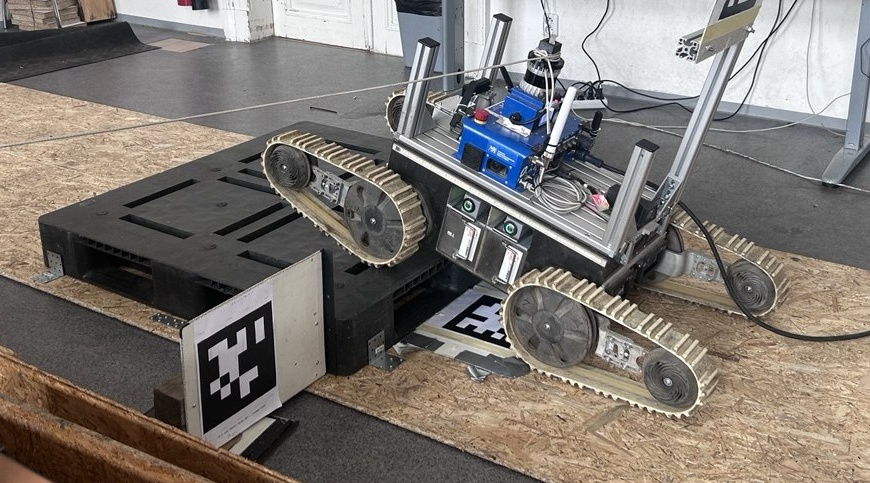
\includegraphics[width=\linewidth]{figures/real_robot_crop.jpg}};
    \node[anchor=north west] (rb) at (ra.south west)
      {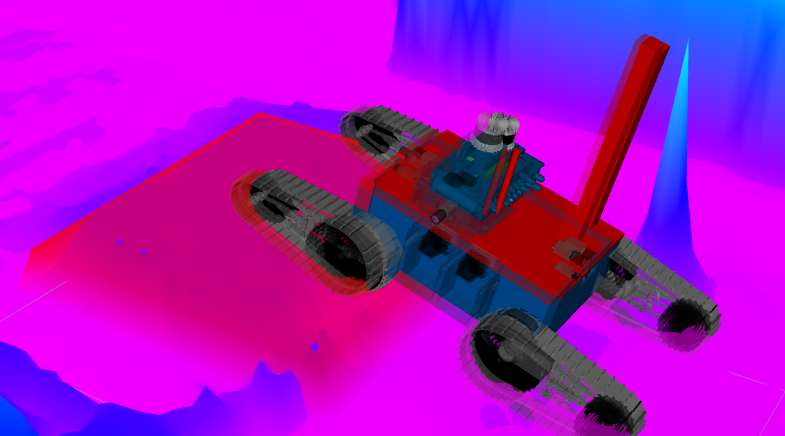
\includegraphics[width=\linewidth]{figures/simulated_robot_crop.png}};
    \node[anchor=north west, inner sep=1.5pt, fill=white, fill opacity=0.75,
          text opacity=1, font=\bfseries\small] at (ra.north west) {(a)};
    \node[anchor=north west, inner sep=1.5pt, fill=white, fill opacity=0.75,
          text opacity=1, font=\bfseries\small] at (rb.north west) {(b)};
  \end{tikzpicture}
  \caption{\textbf{The onboard map against ground truth on a pallet.} (a) The robot climbing a
  pallet obstacle. (b) The same pose, rendered from the data the robot observed there: the
  onboard map (blue) against the handcrafted ground-truth
  map positioned by AprilTags (transparent red), with the ground-truth robot pose drawn
  transparent. The offset between the two surfaces, and between the two bodies, is the map and localization error that the perception stack introduces. The spike behind the robot in the onboard map is a reflected, invalid LiDAR return.}
  \label{fig:robot}
\end{figure}

\textbf{Prior flipper controllers assume an elevation map.}
Across the literature, semi-autonomous and autonomous flipper controllers share a
precondition: they consume an \emph{elevation map} of the terrain under and in front of the
robot as their dominant
input~\cite{chen2023,oehler2024,yuan2019,xu2024,pan2023icm,pan2023atd3qn,ctrac2025,azayev2022}.
Fully manual teleoperation needs no map because the operator sees the terrain from a
third-person view, but must drive all four flippers by hand. 

\textbf{On a real robot, the map is a dead-reckoning artifact.}
Where the estimate of that terrain drifts, due to body occlusion, the commanded flipper
angles are computed for incorrect terrain. Onboard sensors
observe what is ahead, but the body occludes their view of the terrain beneath it.
Dedicated underbody sensors could measure it, but they are rarely fitted and have very
low resolution. That terrain can therefore mainly be \emph{remembered}: observed earlier, accumulated into an elevation
map, and carried beneath the robot as it advances by
\emph{integrating wheel or LiDAR odometry}~\cite{fankhauser2018}. Every stage of this
pipeline is a dead-reckoning process: point-cloud deskewing warps each scan by the estimated
sensor trajectory, and elevation mapping registers successive scans through the
estimated motion~\cite{loam2014}. On the loose, deformable,
step-like terrain where flippers are needed, odometry is least reliable: tracks slip, and
the chassis pitches and drops abruptly, saturating the IMU, and inertial integration cannot
recover the estimate either~\cite{woodman2007imu}. Reflected, invalid LiDAR returns add obstacles that do
not exist, such as the spike behind the robot in Fig.~\ref{fig:robot}.

\textbf{The hardest case is a hidden obstacle.}
When a rigid obstacle is \emph{hidden} (Fig.~\ref{fig:grass}), optical sensors, such as LiDAR or cameras, return the
compliant canopy above it, while the load-bearing obstacle beneath remains invisible until the
chassis stalls on it. Neither a dedicated underbody sensor, which is blinded by the same vegetation, nor foliage-penetrating radar, which is bulky and low-resolution, resolves this in practice.

\textbf{Our contribution: control of the flippers without a map and without an accumulated
pose.}
We present \emph{Stabilizing Anti-Stuck} (\SAS), a reactive controller that requires no
elevation map. It has two terms: a
stabilization term that stabilizes the robot body regardless of the terrain, whether
climbing or descending an obstacle, and an anti-stuck term that frees the robot when it
gets stuck by driving the flippers down. To tell a stuck robot from a moving one, the
anti-stuck term needs a motion cue: a thresholded answer to whether the robot is
moving, which requires neither an accurate nor a metric estimate of the motion. Because the
cue is computed over a short window and is never accumulated, \SAS{} never inherits the drift that corrupts the map. 


\needspace{5\baselineskip}%
\textbf{Contributions:}
\nopagebreak
\begin{enumerate}
  \item We propose \SAS, a mapless flipper controller that needs only a
  thresholded motion cue, combining continuous roll and pitch stabilization with a reactive
  anti-stuck term under a safe directional-priority blend.
  \item We measure the degradation of the elevation map caused by body occlusion and
  odometry drift by evaluating map-based baselines under both a \emph{ground-truth} map and
  the \emph{onboard} map, in a large comparison in simulation of \SAS{} against \emph{twelve}
  map-based baselines and two manual baselines on a twelve-obstacle course; every controller
  drives the full course ten times, with the perception stack reset at each obstacle.
  \item We perform the large comparison on a real obstacle arena with AprilTag ground
  truth: on a four-track robot, each controller drives ten times over a pallet obstacle.
\end{enumerate}


%%%%%%%%%%%%%%%%%%%%%%%%%%%%%%%%%%%%%%%%%%%%%%%%%%%%%%%%%%%%%%%%%%%%%%%%%%%%%%%%
\section{Related Work}\label{sec:related}
% ============================ RELATED WORK ============================
% Structure: manual + three autonomy families (reactive/geometry-based, hierarchical, RL).
Flipper control ranges from manual control to three families of autonomy: reactive and
geometry-based control, hierarchical control, and reinforcement learning.
Table~\ref{tab:sensing} summarizes the compared controllers, their sensing requirements,
and their traversal quality.

\subsection{Manual control}
In direct teleoperation the operator drives the flippers by hand~\cite{cihala2025}, or
switches between preset flipper modes~\cite{larochelle2013,azayev2022}. Manual control
needs no map: the operator observes the terrain, closes the control loop by hand, and also stabilizes
the robot.

\subsection{Reactive and geometry-based control}
A family that computes flipper commands from an explicit terrain model, reactively~\cite{cihala2025}
or by planning, and is the \emph{most} map-dependent of all. Chen et al. combine dynamic programming with a
fast geometry-based pose predictor over the elevation
point cloud~\cite{chen2023}; Yuan et al. plan in the flipper configuration space
from known stair geometry with motion-capture ground truth~\cite{yuan2019}; Oehler
and von Stryk predict pose on a signed-distance field built from
LiDAR~\cite{oehler2024}; and Xu et al. solve a receding-horizon hybrid trajectory
optimization over a simplified terrain sampled from an a priori 3D occupancy map with
FAST-LIO2 odometry~\cite{xu2024}; and, most recently, Zhang et al. plan the path and flipper
maneuvers with RRT* over a contact-model pose predictor, using learned semantic
segmentation of the elevation map only as a perception front-end~\cite{zhang2025}.

\subsection{Hierarchical control}
A family that composes low-level behaviors under a selector. The adaptive-traversability line~\cite{zimmermann2014} classifies
terrain into discrete flipper modes from an elevation map, and for the selected mode a
simple low-level controller drives the flippers. A learned state machine~\cite{azayev2022}
switches among seven hand-crafted flipper morphologies selected from an elevation map. Each
state overlays a \emph{roll}-stabilization term and a stagnation-triggered
\emph{anti-stuck} term that lowers all four flippers to free the robot. It is the one prior
method that couples an anti-stuck term with attitude stabilization, and the origin of the
anti-stuck term we adopt. \TODO{keep this in related work?}

\subsection{Reinforcement learning}
FTR-Bench~\cite{ftrbench2025} standardizes this setting, benchmarking SAC, PPO, TD3, DDPG,
and TRPO on a flipper-track robot in Isaac Lab. Pecka et al. learn a
safety-constrained policy (Constrained REPS) whose state is body pitch plus the terrain
height read from an online octomap~\cite{pecka2016}. Discrete-action variants dominate the
flipper-specific literature: Pan et al. learn a dueling double-DQN over discrete
front/rear flipper increments~\cite{pan2023atd3qn} and extend it with an
intrinsic-curiosity module~\cite{pan2023icm}; both take a local elevation map,
downsampled from a LiDAR point-cloud map built with A-LOAM~\cite{loam2014,aloam}, plus
chassis pitch. Their reward favors smooth pitch only, and getting stuck is a terminal
penalty. Mitriakov et al.
learn staircase negotiation with a policy-gradient method, first from step-edge
geometry with marker-based ground truth~\cite{mitriakov2021} and then in an
open-source Gazebo/ROS framework from depth-image features with ground-truth
pose~\cite{mitriakov2022}, injecting stability through center-of-gravity and
pitch-rate reward shaping. Most recently, C-TRAC learns a contact-aware latent from noisy
LiDAR and drives an asymmetric-SAC policy that, unusually, stabilizes both roll and pitch
via a normalized-energy-stability-margin reward~\cite{ctrac2025}.

\subsection{Attitude stabilization and mapless posture control}\label{sec:related-posture}
Flipper-based attitude stabilization has been studied before, but nearly always on top of
an elevation map: a roll-only stabilization term inside a map-based state
machine~\cite{azayev2022}, and C-TRAC stabilizing both roll and pitch from a reward computed
on the map-based simulator state~\cite{ctrac2025}. Rocha et al.~\cite{rocha2023} regulate
roll, pitch, and ground clearance of an articulated tracked vehicle from the IMU and the
flipper joints alone, but the method is not designed for obstacle traversal. It needs no
exteroceptive sensor and no map, and it is the closest prior work to ours in what it
senses.

\subsection{Evaluating traversal quality}
We evaluate a controller by the quality of the traversal it produces, measured
on the robot's body: IMU-based smoothness such as pitch swing and vertical
shock~\cite{chen2023}, body attitude, and chassis-to-ground clearance.
Following~\cite{cihala2025,zimmermann2014} we score shock, tilt, and clearance
(Sec.~\ref{sec:metrics-block}).

\begin{table*}[t]
\centering
\caption{\textbf{Compared controllers and their traversal quality in Gazebo.} \emph{Map \&
loc.}: needs an onboard map. \emph{Stab.}: attitude axes with an
explicit stabilization objective (r roll, p pitch). \emph{Anti-stuck}: frees itself when
stuck. TQ: mean $\pm$ s.d.\ over ten runs of the twelve-obstacle course under the
ground-truth (GT) and the onboard map; $\Delta$: TQ change under the onboard map;
\emph{Override}: share of obstacle distance the \SAS{} override held the flippers. Manual
rides are driven by an operator at free speed. Best in bold, second best underlined.}
\label{tab:sensing}
\footnotesize
\setlength{\tabcolsep}{2.2pt}
\begin{tabular}{@{}llcccccccc@{}}
\toprule
Controller & Approach & Code & Map \& loc. & Stab. & Anti-stuck & \shortstack{TQ $\uparrow$\\GT map} & \shortstack{TQ $\uparrow$\\onboard map} & $\Delta$ $\uparrow$ & \shortstack{Override [\%] $\downarrow$\\GT / onboard} \\
\midrule
\multicolumn{10}{@{}l}{\emph{Manual}} \\
Manual control~\cite{cihala2025} & direct teleoperation & -- & \xmark & -- & \xmark & -- & 0.612 $\pm$ 0.100 & -- & -- \\
Manual modes~\cite{azayev2022} & operator switches preset modes & -- & \xmark & -- & \xmark & -- & 0.568 $\pm$ 0.101 & -- & -- \\
\midrule
\multicolumn{10}{@{}l}{\emph{Reactive and geometry-based}} \\
{\v C}\'ihala \GC/\OA~\cite{cihala2025} & clearance + obstacle-aware control & released & \cmark & -- & \xmark & \textbf{0.529} $\pm$ 0.011 & 0.486 $\pm$ 0.015 & $-0.043$ & 0.4 / 0.0 \\
Chen GFMP~\cite{chen2023} & pose prediction + dynamic prog. & reimpl. & \cmark & p & \xmark & 0.509 $\pm$ 0.010 & 0.481 $\pm$ 0.012 & $-0.027$ & 7.5 / 8.7 \\
Yuan~\cite{yuan2019} & configuration-space planning & reimpl. & \cmark & -- & \xmark & \underline{0.522} $\pm$ 0.009 & \textbf{0.498} $\pm$ 0.010 & $\underline{-0.024}$ & 11.0 / 8.2 \\
Oehler~\cite{oehler2024} & SDF pose prediction + margin search & released & \cmark & -- & \xmark & 0.499 $\pm$ 0.013 & 0.467 $\pm$ 0.013 & $-0.032$ & 9.9 / 7.1 \\
Xu HTO~\cite{xu2024} & hybrid trajectory optimization & reimpl. & \cmark & p & \xmark & 0.465 $\pm$ 0.007 & 0.439 $\pm$ 0.009 & $-0.026$ & 8.9 / 9.8 \\
Zhang~\cite{zhang2025} & contact-model pose prediction & reimpl. & \cmark & -- & \xmark & 0.493 $\pm$ 0.010 & 0.462 $\pm$ 0.012 & $-0.031$ & 12.7 / 15.2 \\
\midrule
\multicolumn{10}{@{}l}{\emph{Hierarchical}} \\
Azayev~\cite{azayev2022} & learned template state machine & released & \cmark & r & \cmark & 0.436 $\pm$ 0.008 & 0.406 $\pm$ 0.017 & $-0.030$ & 7.1 / 6.7 \\
\midrule
\multicolumn{10}{@{}l}{\emph{Reinforcement learning}} \\
Pecka~\cite{pecka2016} & safety-constrained REPS & reimpl. & \cmark & p & \xmark & 0.458 $\pm$ 0.010 & 0.434 $\pm$ 0.010 & $\underline{-0.024}$ & 7.8 / 9.7 \\
AT-D3QN~\cite{pan2023atd3qn} & dueling double-DQN & reimpl. & \cmark & p & \xmark & 0.473 $\pm$ 0.012 & 0.439 $\pm$ 0.012 & $-0.034$ & 11.4 / 12.7 \\
ICM-D3QN~\cite{pan2023icm} & D3QN + intrinsic curiosity & reimpl. & \cmark & p & \xmark & 0.466 $\pm$ 0.011 & 0.443 $\pm$ 0.009 & $\mathbf{-0.023}$ & 11.2 / 12.9 \\
Mitriakov~\cite{mitriakov2021} & policy-gradient stair climbing & released & \cmark & p & \xmark & 0.451 $\pm$ 0.009 & 0.408 $\pm$ 0.007 & $-0.044$ & 7.3 / 8.3 \\
C-TRAC~\cite{ctrac2025} & contact-aware asymmetric SAC & reimpl. & \cmark & r\&p & \xmark & 0.480 $\pm$ 0.013 & 0.398 $\pm$ 0.008 & $-0.082$ & 0.0 / 7.0 \\
PPO~\cite{sarga2026thesis} & PPO over a heightmap & ours & \cmark & r\&p & \xmark & 0.461 $\pm$ 0.008 & 0.438 $\pm$ 0.010 & $\mathbf{-0.023}$ & 11.7 / 13.7 \\
\midrule
\textbf{\SAS{} (ours)} & attitude stabilization + anti-stuck & ours & \xmark & r\&p & \cmark & \textbf{0.529} $\pm$ 0.008 & \underline{0.497} $\pm$ 0.013 & $-0.032$ & -- \\
\bottomrule
\end{tabular}
\end{table*}



%%%%%%%%%%%%%%%%%%%%%%%%%%%%%%%%%%%%%%%%%%%%%%%%%%%%%%%%%%%%%%%%%%%%%%%%%%%%%%%%
\section{Method}\label{sec:method}
% ============================ METHOD ============================
At every control step \SAS{} reads the body attitude and a motion cue and emits one
velocity per flipper. It pursues two regulation goals: it stabilizes body roll and pitch,
and it releases the robot when it is \emph{stuck}, which means it is commanded forward but
is not advancing. The two terms are formed independently and combined by a
directional-priority rule, so the anti-stuck term can reinforce the stabilization term but
never reverse it.

\SAS{} runs on the four flippers $i\in\{\mathrm{FL},\mathrm{FR},\mathrm{RL},\mathrm{RR}\}$
and emits a per-flipper angular \emph{velocity} command $v_i$. Its inputs are the
gravity-referenced body roll $r$ and pitch $p$ from
the IMU, the four joint angles $\theta_i$, the commanded body velocity $v_\text{cmd}$,
and a scalar motion cue $m$ derived from LiDAR-ICP odometry over a short window
(Sec.~\ref{sec:method-antistuck}).

The command superimposes a stabilization velocity $v^{\mathrm{s}}_i$ and an anti-stuck
velocity $v^{\mathrm{d}}_i$, combined by a directional-priority rule and clamped:
\begin{equation}
  v_i \;=\; \mathrm{limit}\big(\, v^{\mathrm{s}}_i \;+\; \mathrm{cap}(v^{\mathrm{d}}_i,\,v^{\mathrm{s}}_i)\,\big).
  \label{eq:overview}
\end{equation}

\subsection{Attitude stabilization}\label{sec:method-stab}
The dominant term regulates body attitude to level from the IMU alone. The setpoints
$r_0,p_0$ are level, that is zero, and the deviations are $e_r=r_0-r$ and $e_p=p_0-p$. Each
passes through a dead-band of a few degrees, so attitude noise near level produces no
control action. From these we form proportional-integral commands
\begin{equation}
  u_r = K^r_{\mathrm P}\,e_r + K^r_{\mathrm I}\, I_r, \qquad
  u_p = K^p_{\mathrm P}\,e_p + K^p_{\mathrm I}\, I_p,
  \label{eq:pi}
\end{equation}
where $I_{(\cdot)}\!\leftarrow\!\mathrm{clamp}(I_{(\cdot)}+e_{(\cdot)}\Delta t)$ are
anti-windup-limited integrals. The scalar commands map to the four flippers as a front/rear
differential for pitch and a left/right differential for roll:
\begin{equation}
  \begin{bmatrix} v^{\mathrm{s}}_{\mathrm{FL}}\\ v^{\mathrm{s}}_{\mathrm{FR}}\\ v^{\mathrm{s}}_{\mathrm{RL}}\\ v^{\mathrm{s}}_{\mathrm{RR}} \end{bmatrix}
  =
  \begin{bmatrix} -1 & +1\\ -1 & -1\\ +1 & +1\\ +1 & -1 \end{bmatrix}
  \begin{bmatrix} u_p\\ u_r \end{bmatrix}.
  \label{eq:stabmap}
\end{equation}

\subsection{Reactive anti-stuck}\label{sec:method-antistuck}
The subordinate action follows the escape idea of~\cite{azayev2022}: when the robot is
stuck, it drives the flippers to lift the body off the ground and free the robot from the
stuck pose.
It fires whenever the robot is commanded to move yet is not moving:
\begin{equation}
  \text{dig} \;=\; \big(|v_\text{cmd}|>\tau_\text{move}\big)\ \wedge\
  \big(m<\tau_\text{stuck}\big).
  \label{eq:stuck}
\end{equation}
The motion cue $m$ is the standard deviation of the robot's short-horizon displacement
over a sliding window, a \emph{local} measure of whether the body advances, not of where
it is; the window cancels slow drift, so $m$ needs no integrated global pose. It must
measure actual body motion: a track encoder will not do, because a stalled robot can
spin its tracks without advancing. In the current deployment $m$ is the short-window
variance of LiDAR-ICP odometry~\cite{libpointmatcher}. When digging, all
four flippers are driven downward at a lift velocity $\lambda$ so they push against the
terrain and lift the body up, out of the stuck pose; otherwise they retract slowly
toward the flat pose ($-\lambda_\text{low}$):
\begin{equation}
  v^{\mathrm{d}}_i = \begin{cases} +\lambda & \text{dig}\\ -\lambda_\text{low} & \text{otherwise.}\end{cases}
  \label{eq:spread}
\end{equation}
Digging alone can lock up. If the flippers reach their lower position limit without
freeing the robot, the spread the limit permits is zero, the motion cue stays below
$\tau_\text{stuck}$, and the robot would remain stuck indefinitely with its flippers fully
down. A second, longer timer therefore watches the dig itself: after
$T_\text{dig}=\SI{8}{\second}$ of continuous digging without release, the anti-stuck term
is suspended for $T_\text{reset}=\SI{2.5}{\second}$ while the flippers are driven back up
toward the climbing pose, after which digging is permitted again. A dig that cannot free
the robot therefore terminates in a bounded dig--reset cycle rather than a permanent stall.
The reset remains a subordinate demand, so
stabilization still caps it. Stuck detection is armed only after the robot has been
moving for \SI{2}{\second}, so a robot that is merely starting is not mistaken for one that
is stuck.

\subsection{Directional-priority blend and limits}\label{sec:method-blend}
Stabilization takes priority over anti-stuck: the anti-stuck command velocity may reinforce
the stabilization command but must not reverse its direction on any flipper. This is
enforced by the $\mathrm{cap}$ operator, a directional \emph{clamp}: when
$v^{\mathrm{d}}_i$ opposes $v^{\mathrm{s}}_i$ it clamps the anti-stuck command into the band
$[-\alpha|v^{\mathrm{s}}_i|,\,\alpha|v^{\mathrm{s}}_i|]$ set by a fraction $\alpha\in[0,1]$ of the
stabilization demand. It does so only while stabilization is meaningfully active
($|v^{\mathrm{s}}_i|$ above a small dead-band $\beta$), so that attitude noise on a level
robot cannot suppress a dig; otherwise it passes $v^{\mathrm{d}}_i$ through:
\begin{equation}
  \mathrm{cap}(v^{\mathrm{d}}_i,v^{\mathrm{s}}_i)=
  \begin{cases}
    \operatorname{clamp}\big(v^{\mathrm{d}}_i,\ \alpha|v^{\mathrm{s}}_i|\big)
      & \text{if } v^{\mathrm{s}}_i v^{\mathrm{d}}_i<0 \wedge |v^{\mathrm{s}}_i|>\beta,\\[2pt]
    v^{\mathrm{d}}_i & \text{otherwise,}
  \end{cases}
  \label{eq:cap}
\end{equation}
where $\operatorname{clamp}(x,c)$ limits $x$ to $[-c,c]$.



%%%%%%%%%%%%%%%%%%%%%%%%%%%%%%%%%%%%%%%%%%%%%%%%%%%%%%%%%%%%%%%%%%%%%%%%%%%%%%%%
\section{Experiments}\label{sec:experiments}
% ============================ EXPERIMENTS ============================
\subsection{Platform and onboard pipeline}
We evaluate the flipper controllers both in simulation and on the real platform. The onboard perception pipeline that the map-based baselines
consume is representative of current practice: an Ouster LiDAR and IMU feed point-cloud
deskewing and LiDAR-ICP odometry~\cite{norlabicpmapper,libpointmatcher}, which drive elevation
mapping~\cite{fankhauser2018} to produce a robot-centric
elevation map, which we call the \emph{onboard map}.

\paragraph{Simulation comparison} We simulate in Gazebo~\cite{gazebo2004}, the simulator selected
for the virtual track of the DARPA Subterranean Challenge~\cite{roucek2022subt}. Unlike
typical simulators that approximate tracks with multiple wheels, we employ the track
simulation of~\cite{pecka2017tracks}, which models conveyor-belt behavior. The sensors match the real payload: a simulated Ouster OS0
($1024\times64$ rays at \SI{10}{\hertz}, \SIrange{0.1}{50}{\metre}, \SI{1}{\centi\metre}
Gaussian range noise) and a \SI{50}{\hertz} IMU with Gaussian noise and a slowly varying
bias. The simulation runs the same ROS~2 nodes as the real robot, so the onboard-map condition
runs the same ICP and elevation-mapping stack on these noisy streams; the ground-truth condition reads pose and map from the
simulator. The arena is the twelve-obstacle warehouse course of~\cite{cihala2025}
(Fig.~\ref{fig:obstacles}): a straight aisle lined with twelve numbered obstacles of
variable difficulty, including pallets, stacked boxes, planks, and a staircase.

\paragraph{Real robot comparison} The real arena repeats the protocol on one pallet obstacle between
two reset zones (Fig.~\ref{fig:robot}). AprilTag markers on the robot and in the arena,
seen by a camera on a stand, give an absolute localization that registers the handcrafted
ground-truth map.

\paragraph{Automated ride and \SAS{} override} In all reported runs the robot is
driven autonomously. A ride node drives the robot at a constant
\SI{0.6}{\metre\per\second} in simulation and, for safety, \SI{0.25}{\metre\per\second}
on the real robot. A controller that stalls inside a field is released
by the \emph{\SAS{} override}, which hands the flippers to \SAS{} until the robot moves
again, and the field is finished. A field not left
within \SI{120}{\second} is scored as not traversed.

\subsection{Baselines}
We compare against, in increasing autonomy: (i) \textbf{Manual control}, an expert
operator driving all four flippers by hand (the traversal-quality
ceiling~\cite{cihala2025}), and \textbf{Manual modes}, the operator switching between
preset flipper modes by hand~\cite{azayev2022}; (ii) the \textbf{\GC/\OA{}
controller}~\cite{cihala2025} in its automated form, where instead of the operator a
\SI{2}{\second} stuck timer switches the front flippers between \OA{} and \GC{}; (iii) every map-based controller catalogued in
Table~\ref{tab:sensing}; and our \textbf{\SAS}. Where the authors released code we run their
implementation; where they did not, we use our reimplementation from the paper, adapted
to a four-track robot. The geometry-based controllers were
adapted to the four-track morphology as follows. Chen's GFMP~\cite{chen2023} keeps the
exact two-contact solver and waypoint DP, but admits only flipper-supported contact cases,
since the chassis is passive, adds an absolute-pitch levelness cost, and uses the
four-track geometry and elevation-map profile. Yuan's configuration-space
planner~\cite{yuan2019} was reimplemented for the four-track link geometry, estimating step distance and height per tick from the onboard elevation
map instead of motion capture, replanning closed-loop and holding where the model is
undefined. Oehler and von Stryk's pose predictor~\cite{oehler2024}, given a four-flipper model
with a passive belly, gains the selection stage it lacks: a
43-candidate sweep commanding the highest-stability-margin configuration, holding when
no configuration is stable. Xu's HTO~\cite{xu2024} assumes a driven belly that carries the step edge;
with a passive belly the belly-contact regimes of its hybrid model are replaced on ascents by a
double-prop flipper bridge with enforced belly clearance, plus rear-release and
descent-preparation schedules. Zhang's planner~\cite{zhang2025} is reproduced only as its
contact-model pose prediction and action cost, solved at a virtual station
\SI{0.5}{\metre} ahead; chassis-supported poses are
forbidden on the passive belly.

\begin{figure*}[t]
  \centering
  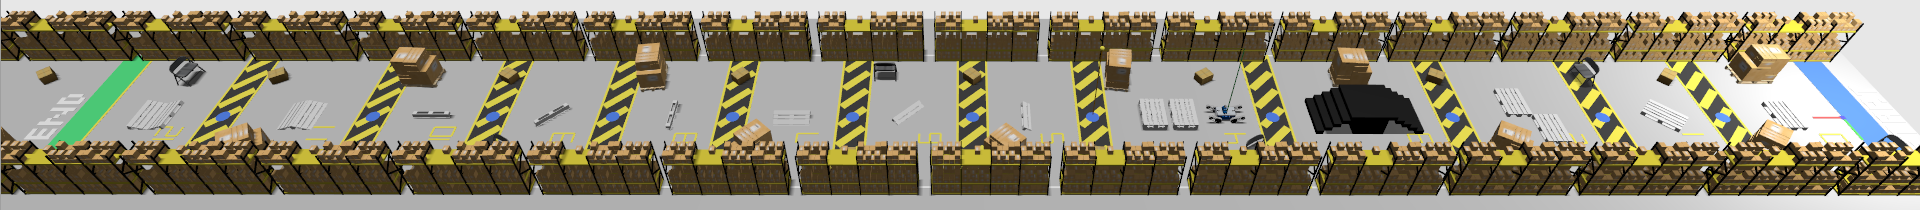
\includegraphics[width=\textwidth]{figures/gazebo_arena}
  \caption{\textbf{Automated simulation arena.} The Gazebo warehouse course
  of~\cite{cihala2025}: a straight aisle of twelve numbered obstacles of variable
  difficulty, each probing a different controller capability (pallets, stacked
  boxes, planks, and a staircase); the robot starts at the right. In the automated
  ride (Sec.~\ref{sec:experiments}) it is driven at a constant
  \SI{0.6}{\metre\per\second} through every field in turn, with a \SI{1}{\metre}
  settling strip between fields and a \SI{120}{\second} timeout per field.}
  \label{fig:obstacles}
\end{figure*}

\subsection{Ground-truth map for a fair baseline}
Our claim is that the onboard map is the limiting input, so evaluating the map-based
baselines under that map alone would conflate the controller with its perception. We
therefore run each of them twice:
once with the onboard map, and once with a \emph{ground-truth} map
that removes odometry drift. The gap between a
baseline's two scores measures its sensitivity to onboard mapping.

\subsection{Metrics}
Following~\cite{cihala2025} we report \textbf{traversal quality} (TQ), the mean of three
normalized sub-metrics: (a) \emph{acceleration/shock} $s$ from the IMU, (b) body
\emph{tilt} (roll/pitch magnitude), and (c) \emph{ground clearance}. All three are
computed against ground truth: in simulation the reference pose and map are read directly
from the simulator; on the real robot they come from external localization and a
handcrafted elevation map of the obstacle. The clearance score penalizes the deviation of the chassis clearance from its flat-ground
value outside a dead-band, linearly up to belly contact and \SI{10}{\centi\metre} above.
Rewarding raw clearance would favor baselines that freeze their flippers and coast in a
high pose.
\label{sec:metrics-block}%
Each channel is reduced over a traversal by a \emph{distance-binned maximum}. We bin by distance because we compare quality across the
obstacle, while each controller takes a different time to traverse it: every \SI{0.25}{\metre} of obstacle forms one bin, the
worst normalized sample in each bin is taken, and the bins are averaged; a field not
traversed scores $\mathrm{TQ}{=}0$. The raw streams are not low-pass filtered: shock is
the acceleration magnitude $|a|$ from the IMU at \SI{21}{\hertz}, normalized by
$N(s,s_{\max}/2)$~\cite{cihala2025}, with $s_{\max}=\SI{57.5}{\metre\per\second\squared}$
on the real robot and $s_{\max}=\SI{197}{\metre\per\second\squared}$ in Gazebo; clearance is the
closest ground point of a $10\times8$ grid on \SI{5}{\centi\metre} spacing under the
chassis. The three channels measure different things: over the traversed Gazebo
obstacles their pairwise Spearman correlations are $0.26$ (shock--clearance), $0.28$
(shock--tilt) and $0.39$ (clearance--tilt), and over the real crossings $0.06$, $0.39$ and
$-0.03$.

\begin{table*}[t]
\centering
\caption{\textbf{Traversal quality in Gazebo and on the real pallet.} Gazebo: mean over ten runs
of the twelve-obstacle course. Real: one ride of ten crossings per controller and map, mean over
the crossings, a crossing not completed scoring zero. All channels are scored against ground
truth, with $s_{\max}$ \SI{197}{\metre\per\second\squared} in Gazebo and
\SI{57.5}{\metre\per\second\squared} on the real robot. $\Delta$: TQ change under the onboard
map. \emph{Overrides}: activations of the \SAS{} override, per twelve-obstacle course in Gazebo
(mean over runs) and per ten-crossing ride on the real robot. Manual rides are hand-driven.
Best TQ in bold, second best underlined.}
\label{tab:results}
\footnotesize
\setlength{\tabcolsep}{3pt}
\begin{tabular*}{\textwidth}{@{\extracolsep{\fill}}lcccccccc@{}}
\toprule
 & \multicolumn{4}{c}{Gazebo, twelve obstacles} & \multicolumn{4}{c}{Real pallet, one ride of ten crossings} \\
\cmidrule(lr){2-5}\cmidrule(l){6-9}
Controller & \shortstack{TQ $\uparrow$\\GT map} & \shortstack{TQ $\uparrow$\\onboard map} & $\Delta$ $\uparrow$ & \shortstack{Overrides $\downarrow$\\GT / onboard} & \shortstack{TQ $\uparrow$\\GT map} & \shortstack{TQ $\uparrow$\\onboard map} & $\Delta$ $\uparrow$ & \shortstack{Overrides $\downarrow$\\GT / onboard} \\
\midrule
\multicolumn{9}{@{}l}{\emph{Manual}} \\
Manual control~\cite{cihala2025} & -- & 0.867 & -- & -- & -- & 0.810 & -- & -- \\
Manual modes~\cite{azayev2022} & -- & 0.825 & -- & -- & -- & 0.810 & -- & -- \\
\midrule
\multicolumn{9}{@{}l}{\emph{Reactive and geometry-based}} \\
{\v C}\'ihala \GC/\OA~\cite{cihala2025} & 0.800 & 0.780 & $-0.020$ & 0.1 / 0.0 & 0.612 & 0.657 & $+0.045$ & 0 / 0 \\
Chen GFMP~\cite{chen2023} & \underline{0.807} & \underline{0.787} & $-0.021$ & 5.0 / 6.2 & 0.660 & 0.661 & $+0.001$ & 10 / 10 \\
Yuan~\cite{yuan2019} & 0.807 & 0.783 & $-0.024$ & 7.3 / 5.9 & \underline{0.710} & \textbf{0.721} & $+0.012$ & 4 / 3 \\
Oehler~\cite{oehler2024} & 0.801 & 0.774 & $-0.028$ & 6.9 / 5.1 & 0.591 & 0.651 & $+0.060$ & 9 / 4 \\
Xu HTO~\cite{xu2024} & 0.783 & 0.768 & $-0.014$ & 6.0 / 5.9 & 0.685 & 0.677 & $-0.008$ & 10 / 10 \\
Zhang~\cite{zhang2025} & 0.790 & 0.774 & $-0.016$ & 7.4 / 9.0 & 0.689 & 0.693 & $+0.004$ & 10 / 10 \\
\midrule
\multicolumn{9}{@{}l}{\emph{Hierarchical}} \\
Azayev~\cite{azayev2022} & 0.763 & 0.746 & $-0.017$ & 4.6 / 4.2 & 0.662 & 0.694 & $+0.032$ & 0 / 0 \\
\midrule
\multicolumn{9}{@{}l}{\emph{Reinforcement learning}} \\
Pecka~\cite{pecka2016} & 0.781 & 0.765 & $-0.016$ & 6.0 / 6.7 & 0.642 & 0.640 & $-0.003$ & 0 / 0 \\
AT-D3QN~\cite{pan2023atd3qn} & 0.784 & 0.768 & $-0.016$ & 6.7 / 7.6 & 0.642 & 0.644 & $+0.002$ & 9 / 1 \\
ICM-D3QN~\cite{pan2023icm} & 0.779 & 0.770 & $-0.009$ & 6.5 / 7.7 & 0.652 & 0.548 & $-0.104$ & 10 / 14 \\
Mitriakov~\cite{mitriakov2021} & 0.778 & 0.752 & $-0.026$ & 5.2 / 5.6 & \textbf{0.712} & 0.635 & $-0.077$ & 0 / 5 \\
C-TRAC~\cite{ctrac2025} & 0.789 & 0.680 & $-0.110$ & 0.0 / 16.0 & 0.457 & 0.478 & $+0.020$ & 18 / 17 \\
PPO~\cite{sarga2026thesis} & 0.780 & 0.768 & $-0.012$ & 7.7 / 8.5 & 0.647 & 0.647 & $0.000$ & 0 / 0 \\
\midrule
\textbf{\SAS{} (ours)} & \textbf{0.813} & \textbf{0.793} & $-0.020$ & -- & 0.680 & \underline{0.703} & $+0.023$ & -- \\
\bottomrule
\end{tabular*}
\end{table*}

\subsection{Results}
Table~\ref{tab:results} reports TQ per controller in Gazebo under the ground-truth and
the onboard map, and how often the \SAS{} override had to release each controller. Every controller, \SAS{} included, loses quality under the onboard map, by
$0.01$ to $0.03$ (C-TRAC by $0.11$); \SAS{}, which reads no map, loses $0.020$ through its
LiDAR-ICP odometry cue alone, and frees itself without the \SAS{} override, which releases
the map-based controllers 4 to 9 times per course under either map. C-TRAC degrades the most
under the onboard map, by $0.11$, and shows most clearly that the onboard map raises the need
for the override: never overridden under the ground-truth map, it is released 16 times per
course under the onboard map; Chen, Zhang, Pecka, AT-D3QN, ICM-D3QN and PPO also need more
releases under the onboard map, Yuan, Oehler and Azayev fewer.
Sampled over the body footprint (the chassis and \SI{1.5}{\metre} ahead, at
\SI{5}{\centi\metre}) every \SI{0.25}{\second}, the height difference between the onboard
and the ground-truth map has a median absolute value of \SI{0.9}{\centi\metre} and a median
per-snapshot RMSE of \SI{2.6}{\centi\metre}, with 4\% of the cells off by more than
\SI{10}{\centi\metre}.
The onboard map also reports its own uncertainty, and in Gazebo it grows over every
obstacle: the median bound width of the cells under the body rises from
\SI{2.4}{\centi\metre} at the reset to \SIrange{4.5}{4.9}{\centi\metre} after
\SI{8}{\second} on the obstacle, and its 90th percentile from \SI{3}{\centi\metre} to
\SIrange{17}{20}{\centi\metre}, the occluded cells the controllers regulate on. On the real
robot the mapper's per-cell variance shrinks with fusion, from \SI{1}{\centi\metre} to
\SI{3}{\milli\metre}, and does not reflect the map error. In one
C-TRAC run under the ground-truth map the robot tipped over on obstacle~7, the only
tip-over in either campaign; that obstacle is scored as not traversed.

On the real pallet (Table~\ref{tab:results}) the operator remains the reference: manual
control and manual modes both score $0.81$, above every controller. Among the
controllers, Yuan and \SAS{} lead under the onboard map at $0.70$--$0.72$, Mitriakov and Yuan
under the ground-truth map at $0.71$, and with one ride per condition the difference between
the two maps is within the spread over crossings for most of them. \SAS{} is never
overridden and completes every crossing; the map-based
controllers that stall are released by the \SAS{} override up to 18 times per ride (C-TRAC),
and C-TRAC and ICM-D3QN abort crossings under either map. The largest degradations under the onboard map are
ICM-D3QN ($-0.10$) and Mitriakov ($-0.08$). Unlike in Gazebo, the onboard map does not raise the
number of releases on the real robot for most controllers: AT-D3QN drops from 9 to 1 per ride
and Oehler from 9 to 4, Chen, Xu, Zhang and C-TRAC stay at their level, and only ICM-D3QN
(10 to 14) and Mitriakov (0 to 5) need more. The tilt channel, the target of
the stabilization term, is where \SAS{} leads: $0.86$ in Gazebo, level with Chen and ahead of
the rest ($0.75$--$0.85$), and on the real pallet its maximum tilt over the ride is
\ang{11.5}, against \ang{12} to \ang{26} for the other controllers and \ang{36} for C-TRAC.


%%%%%%%%%%%%%%%%%%%%%%%%%%%%%%%%%%%%%%%%%%%%%%%%%%%%%%%%%%%%%%%%%%%%%%%%%%%%%%%%
\section{Conclusion}\label{sec:conclusion}
% ============================ CONCLUSION ============================
State-of-the-art flipper controllers depend on an elevation map of the occluded ground under
the chassis, which drifts with odometry on exactly the terrain where flippers are needed.
\SAS{} removes that dependency: its stabilization term regulates roll and pitch from the
IMU, and its anti-stuck term, triggered by a short-window odometry cue, frees the robot when
stuck; a directional-priority blend keeps stabilization in control. It cannot anticipate an obstacle before contact,
but it keeps the robot stabilized and operational where the onboard map, and with it every
map-based controller, breaks down.

Future work targets a more robust odometry cue by fusing LiDAR-ICP odometry with camera
odometry or integrated IMU motion, which should hold up in the occluded, feature-poor, or
flat places where ICP alone struggles, and a fallback scheme that defers to a map-based
controller when the onboard map is trustworthy and to \SAS{} when it is not.


%%%%%%%%%%%%%%%%%%%%%%%%%%%%%%%%%%%%%%%%%%%%%%%%%%%%%%%%%%%%%%%%%%%%%%%%%%%%%%%%
\bibliographystyle{IEEEtran}
\bibliography{root}

\end{document}
